% !TEX root = ../my-thesis.tex
%
\chapter{Appendix}
\label{sec:appendix}
% LTEX: enabled=false
\lstset{
  breakatwhitespace=true,
  breaklines=true,
  breakindent=0pt,
  numbers=none
}
% LTEX: enabled=true

\section{Datasets}
\label{sec:appendix:datasets}
For the experiments conducted in this thesis, group-specific answers from different sources have been utilized, as described in Section~\ref{sec:datasets}. These answers were divided into training, validation, and test sets to fine-tune various models. Within each of these splits, the groups were represented equally to ensure balanced training and evaluation conditions.

\begin{tblr}{llS[table-format=5.0,group-minimum-digits=4]S[table-format=4.0]}
  \toprule
  {Purpose}             & {Dataset}      & {Number of Answers} & {Answers per Group} \\
  \midrule
  \acs{sfam} train      & Stack Exchange & 4400                & 400                 \\
  \acs{sfam} validation & Stack Exchange & 550                 & 50                  \\
  \acs{sfam} test       & Stack Exchange & 550                 & 50                  \\
  \acs{lisa} train      & Stack Exchange & 55000               & 5000                \\
  \acs{lisa} validation & Stack Exchange & 3300                & 300                 \\
  \acs{lisa} test       & Stack Exchange & 2200                & 200                 \\
  foreign domain test   & AskX           & 3500                & 500                 \\
  \bottomrule
\end{tblr}

In addition to the datasets used for training and evaluation, a total of \num{400} questions were employed in the steering experiments presented in Section~\ref{sec:datasets:steering}. Of these questions, \num{320} were sourced from the work of \citet{petroni-etal-2021-kilt}, while the remaining \num{80} questions were taken from the work of \citet{rooeinKnowYourAudience2023}.

\clearpage

\subsection{Stack Exchange}
\label{sec:appendix:datasets:stackex}
In the following table, all groups that were extracted from Stack Exchange and the number of answers to what/how/why questions are listed.

\begin{tblr}{
    colspec={ X S[table-format=5.0,group-minimum-digits=4] S[table-format=4.0] },
  }
  \toprule
  {Group}              & {Answers Total} & {Answers Used} \\
  \midrule
  Astronomers          & 3955            & 0              \\
  Pilots               & 12315           & 6000           \\
  Biologists           & 6438            & 6000           \\
  Chemists             & 8131            & 6000           \\
  Cryptographers       & 5185            & 0              \\
  Computer Scientists  & 6364            & 6000           \\
  Data Scientists      & 4262            & 0              \\
  Electrical Engineers & 21506           & 6000           \\
  Game Developers      & 10835           & 6000           \\
  Historians           & 7176            & 6000           \\
  Lawyers              & 5148            & 0              \\
  Mechanical Engineers & 3682            & 0              \\
  Philosophers         & 8554            & 6000           \\
  Physicists           & 46193           & 6000           \\
  Politicians          & 12855           & 6000           \\
  Software Engineers   & 31840           & 6000           \\
  \bottomrule
\end{tblr}

\vfill
\clearpage

\subsection{Reddit (AskX)}
\label{sec:appendix:datasets:askx}
\vspace{-3mm}
The following table presents an overview of the Subreddits from which the answers used for the experiments in this thesis were sourced. It also includes information on the number of answers to what/how/why questions extracted from each Subreddit. Furthermore, the table illustrates how the Subreddits were grouped. Finally, it specifies the number of answers that were actually utilized in the experiments, which is \num{500} in total per group.
  % LTEX: enabled=false
  {
    \small

    \begin{tblr}{
        colspec={ X X S[table-format=4.0] S[table-format=3.0] },
      }
      \toprule
      {Group}                            & {Subreddit}        & {Answers Total} & {Answers Used} \\
      \midrule
      \SetCell[r=3]{m} Computer          & Askcomputerscience & 169             & 144            \\
                                         & Askprogrammers     & 114             & 99             \\
                                         & Askprogramming     & 289             & 257            \\
      \midrule
      \SetCell[r=8]{m}   Engineering     & Askamechanic       & 9               & 5              \\
                                         & Askanengineer      & 31              & 21             \\
                                         & Askelectricians    & 15              & 11             \\
                                         & Askelectronics     & 45              & 31             \\
                                         & Askengineers       & 580             & 404            \\
                                         & Askmechanics       & 15              & 11             \\
                                         & Asktechnology      & 11              & 7              \\
                                         & Askanelectrician   & 12              & 10             \\
      \midrule
      \SetCell[r=4]{m}   Natural Science & Askbiology         & 166             & 142            \\
                                         & Askchemistry       & 89              & 74             \\
                                         & Askphysics         & 331             & 282            \\
                                         & Askachemist        & 2               & 2              \\
      \midrule
      Old                                & Askoldpeople       & 8769            & 500            \\
      \midrule
      \SetCell[r=4]{m}  Over30           & Askmenover30       & 2242            & 178            \\
                                         & Askmenover40       & 163             & 17             \\
                                         & Askwomenover30     & 3105            & 235            \\
                                         & Askwomenover40     & 724             & 70             \\
      \midrule
      \SetCell[r=3]{m}  Social           & Asksocialscience   & 227             & 134            \\
                                         & Askapsychologist   & 68              & 45             \\
                                         & Askpsychology      & 500             & 321            \\
      \midrule
      \SetCell[r=3]{m}   Teenager        & Askteengirls       & 318             & 138            \\
                                         & Askteens           & 307             & 143            \\
                                         & Askteenboys        & 551             & 219            \\
      \bottomrule
    \end{tblr}
  }
% LTEX: enabled=true

\clearpage

\section{Prompts for Attribute Sentence Generation}
The following prompts are used to create the synthetic dataset (see Section~\ref{sec:approach:attributeSentenceGeneration}). Many of the prompts have been taken from the work of \citet{patelLearningInterpretableStyle2023} with the notable exception of the knowledge prompts, which are part of the extension to the existing approach presented in this thesis.

\subsection{Open-ended Style Prompts}
\label{sec:appendix:openPrompts}
\begin{description}
  \item[Grammar Style]\leavevmode \newline
        \begin{minipage}{\linewidth}
          \begin{lstlisting}
Write a long paragraph describing the unique grammar style of the following passage without referring to specifics about the topic.
Passage: {{passage}}
Description:
\end{lstlisting}
        \end{minipage}
  \item[Vocabulary Style]\leavevmode \newline
        \begin{minipage}{\linewidth}
          \begin{lstlisting}
Write a long paragraph describing the unique vocabulary style of the following passage without referring to specifics about the topic.
Passage: {{passage}}
Description:
\end{lstlisting}
        \end{minipage}
  \item[Punctuation Style]\leavevmode \newline
        \begin{minipage}{\linewidth}
          \begin{lstlisting}
Write a long paragraph describing the unique punctuation style of the following passage without referring to specifics about the topic.
Passage: {{passage}}
Description:
\end{lstlisting}
        \end{minipage}
  \item[Grammar Errors]\leavevmode \newline
        \begin{minipage}{\linewidth}
          \begin{lstlisting}
Write a long paragraph describing the grammar errors (if any) of the following passage without referring to specifics about the topic.
Passage: {{passage}}
Description:
\end{lstlisting}
        \end{minipage}
  \item[Spelling Errors]\leavevmode \newline
        \begin{minipage}{\linewidth}
          \begin{lstlisting}
Write a long paragraph describing the spelling errors (if any) of the following passage without referring to specifics about the topic.
Passage: {{passage}}
Description:
\end{lstlisting}
        \end{minipage}
  \item[Forensic Linguistics]\leavevmode \newline
        \begin{minipage}{\linewidth}
          \begin{lstlisting}
Write a long paragraph describing the unique stylometric features of the following passage without referring to specifics about the topic from the perspective of a forensic linguist psychoanalyzing the writer.
Passage: {{passage}}
Description:
\end{lstlisting}
        \end{minipage}
\end{description}

\subsection{Targeted Style Prompts}
\label{sec:appendix:targetPrompts}

In this thesis, the following template for the targeted style prompts are being used:
\begin{lstlisting}
  Write a description about the usage of '{{feature_name}}' by the author of the following passage. If it is used by the author write a long description, otherwise keep the answer short.
  Passage: {{passage}}
  Description:
\end{lstlisting}

For each of the following targeted features, the \textit{feature\_name} is substituted by the feature name. The list of features follows the work of \citet{patelLearningInterpretableStyle2023} with the exception that \enquote{swear words} is not included twice and \enquote{male pronouns} as well as \enquote{female pronouns} have been removed because the resulting attribute sentences are too similar to each other. Because of the high similarity, the attributes were often in the same clusters, even though they were describing different genders.

% LTEX: enabled=false
\begin{multicols}{2}
  \begin{itemize}[nolistsep]
    \item figurative language
    \item sarcasm
    \item sentence fragment
    \item run-on sentences
    \item active voice
    \item passive voice
    \item agreement errors
    \item prosocial behaviors
    \item antisocial behaviors
    \item being polite
    \item showing interpersonal conflict
    \item moralizing
    \item communication words
    \item indicators of power
    \item talk of achievement
    \item indication of certitude
    \item being tentative
    \item insight
    \item all or none thinking
    \item words related to memory
    \item positive emotion
    \item negative emotion
    \item anxiety
    \item anger
    \item sadness
    \item positive tone
    \item negative tone
    \item neutral tone
    \item words related to auditory perception
    \item words related to visual perception
    \item words related to space perception
    \item words related to motion perception
    \item words related to attention
    \item words related to allure
    \item words related to curiosity
    \item words related to risk
    \item words related to reward
    \item words expressing needs
    \item words expressing wants
    \item words expressing acquisition
    \item words expressing lack
    \item words expressing fulfillment
    \item words expressing fatigue
    \item words expressing illness
    \item words expressing wellness
    \item words related to mental health
    \item words related to food or eating
    \item words related to death
    \item words related to self-harm
    \item sexual content
    \item words related to leisure
    \item words related to home
    \item words related to work
    \item words related to money
    \item words related to religion
    \item words related to politics
    \item words related to culture
    \item swear words
    \item foreign words
    \item scholarly words
    \item slang words
    \item social media slang words
    \item filler words
    \item words focusing on the past
    \item words focusing on the present
    \item words focusing on the future
    \item words related to time
    \item misspelled words
    \item repeated words
    \item words expressing quantity
    \item words indicating family
    \item words indicating friends
    \item words indicating men
    \item words indicating women
    \item words indicating pets
    \item words indicating social status
    \item words indicating poverty
    \item words indicating wealth
    \item punctuation symbols
    \item hyphenated words
    \item oxford comma
    \item parentheticals
    \item numbers
    \item elongated words
  \end{itemize}
\end{multicols}
% LTEX: enabled=true

\subsection{Knowledge Prompts}
\label{sec:appendix:knowledgePrompts}
\begin{description}
  \item[Experience]\leavevmode \newline
        \begin{minipage}{\linewidth}
          \begin{lstlisting}
Write a description of the experience the author has based on the following passage.
Passage: {{passage}}
Description:
\end{lstlisting}
        \end{minipage}
  \item[Background Knowledge]\leavevmode \newline
        \begin{minipage}{\linewidth}
          \begin{lstlisting}
Write a description of the background knowledge the author has based on the following passage.
Passage: {{passage}}
Description:
\end{lstlisting}
        \end{minipage}
\end{description}

% TODO:
% \section{Steered Explanations}
% These are two example of explanation that were generated by a steered \ac{llm}.

\section{Database Schema}
\label{sec:appendix:databaseSchema}
All the data used in this thesis has been consolidated into a single SQLite database. This centralized storage solution allows for easier access to and manipulation of the various datasets, annotations, and intermediate representations generated throughout the research process.

The resulting database file is approximately \SI{12}{\giga\byte} in size. Its size reflects the comprehensive nature of the stored information, including the synthetic dataset, model outputs, attribute vectors, and metadata relevant to group-specific explanations and experimental results.

The datasets presented in Section~\ref{sec:datasets} have been saved in the database to the extent that they were used in this thesis. In particular, the Stack Exchange and AskX datasets have been stored in the tables named \textit{questions} and \textit{answers}, though only the answers were used directly for the experiments. The steering questions, which are central to the evaluation of the steering techniques proposed in this work, are recorded in the table \textit{steering\_questions}. Finally, the table named \textit{meta} exists solely to ensure compatibility with programs that interact with the database. It helps verify that the configuration and number of data samples align with the conditions under which the database was created. The \textit{meta} column names correspond to the values in the \enquote{data\_type} column of the \textit{answer} table.

\begin{center}
  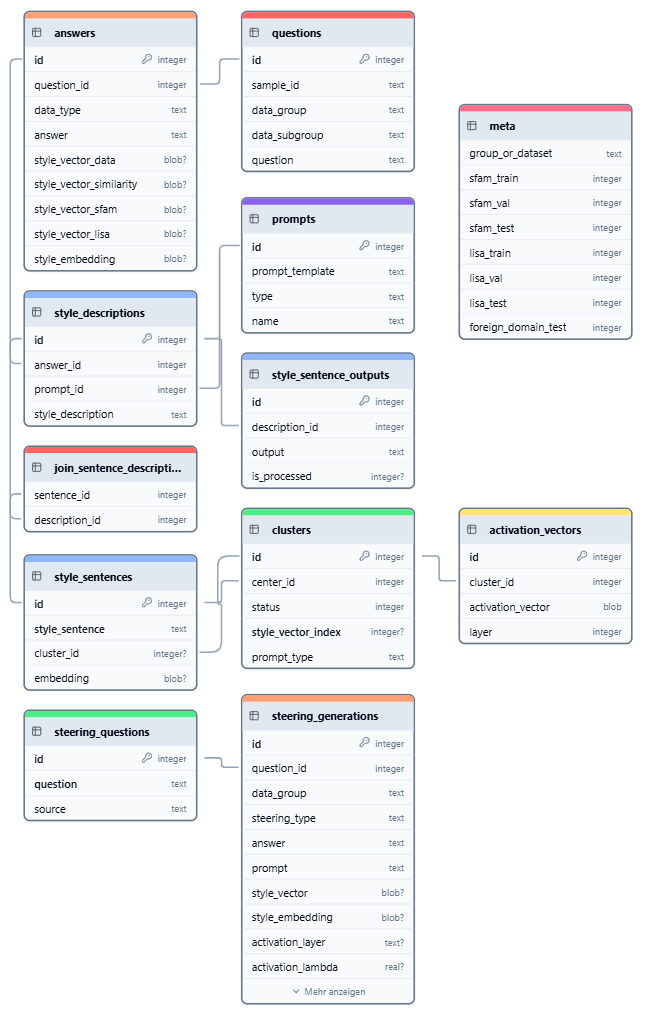
\includegraphics[width=\linewidth]{figures/sqlite-db.png}
\end{center}
